\documentclass{beamer}

\usepackage[utf8]{inputenc}
\usepackage{graphicx}
\usepackage{amsmath}
\usepackage{hyperref}
\usepackage{tikz}
\usetikzlibrary{shapes,arrows.meta,positioning}
\usetikzlibrary{quantikz2}

\title{\Large{Response to Ramesh \& Vinay, (2003)} \\
\small{\texorpdfstring{\textit{String Matching in \(\tilde{O}(\sqrt{n} + \sqrt{m})\) Quantum Time}}{String Matching in O(sqrt(n) + sqrt(m)) Quantum Time}}
}
\author{Matthew Evans, Ariz Siddiqui, Nathan Puskuri}
\date{\today}

\begin{document}

\begin{frame}
    \titlepage
\end{frame}

\begin{frame}{Outline}
    \tableofcontents
\end{frame}

\section{Introduction}
\begin{frame}{\texorpdfstring{\textit{String Matching in \(\tilde{O}(\sqrt{n} + \sqrt{m})\) Quantum Time}}{String Matching in O(sqrt(n) + sqrt(m)) Quantum Time}}
    \normalsize
    H.\ Ramesh \& V.\ Vinay (IISc Bangalore, 2000)\\
    \vfill
    \begin{block}{Problem Statement}
        Given a text $t$ of length $n$ and a pattern $p$ of length $m$, decide whether $p$ occurs in $t$.
    \end{block}
    \vfill
    \begin{itemize}
        \item \textbf{Classical bound:} $\Theta(n + m)$ via KMP, Boyer-Moore, etc.
        \item \textbf{Quantum goal:} Exploit amplitude amplification to beat linear time.
        \item \textbf{Main result:} A quantum algorithm running in
              \[
                  \widetilde{O}\bigl(\sqrt{n} + \sqrt{m}\bigr)
              \]
              with constant two-sided error probability.
    \end{itemize}
\end{frame}


\begin{frame}
    \begin{figure}
        \centering
        \resizebox{1\textwidth}{!}{%
            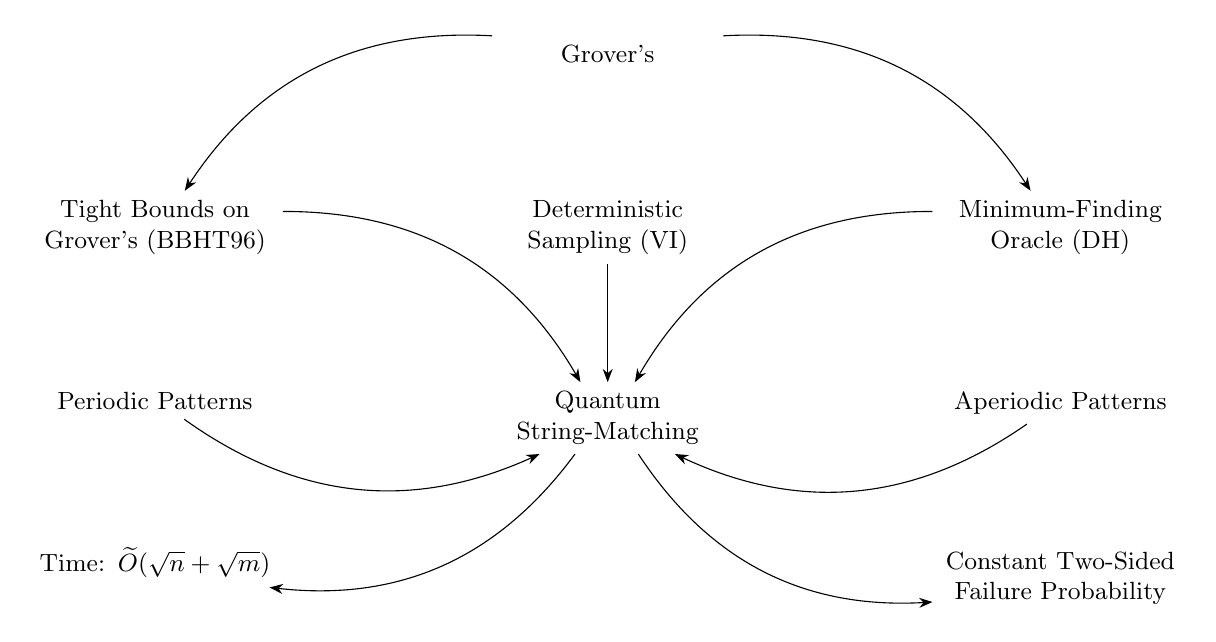
\begin{tikzpicture}[
                scale=0.8,
                >={Stealth[]},
                every node/.style={font=\small, text width=3cm, align=center},
                node distance=1.5cm and 2.5cm
                ]
                % Nodes with plain text only
                \node (proposed)  {Quantum String-Matching};
                \node (vi)       [above=of proposed]      {Deterministic Sampling (VI)};
                \node (grover)   [above=of vi]            {Grover's};
                \node (bbht)     [below left=of grover]   {Tight Bounds on Grover's (BBHT96)};
                \node (dh)       [below right=of grover]  {Minimum-Finding Oracle (DH)};
                \node (aper)     [below=of dh]            {Aperiodic Patterns};
                \node (periodic) [below=of bbht]          {Periodic Patterns};
                \node (time)     [below=of periodic]      {Time: $\widetilde{O}(\sqrt{n}+\sqrt{m})$};
                \node (prob)     [below=of aper]          {Constant Two-Sided Failure Probability};

                % Curvy edges
                \draw[->, bend right]  (grover)   to (bbht);
                \draw[->, bend left]   (grover)   to (dh);
                \draw[->, bend left]   (bbht)     to (proposed);
                \draw[->, bend right]  (dh)       to (proposed);
                \draw[->]              (vi)       to (proposed);
                \draw[->, bend left]   (aper)     to (proposed);
                \draw[->, bend right]  (periodic) to (proposed);
                \draw[->, bend left]   (proposed) to (time);
                \draw[->, bend right]  (proposed) to (prob);
            \end{tikzpicture}%
        }
        \caption{Conceptual dependencies in the $\widetilde{O}(\sqrt{n}+\sqrt{m})$ quantum string-matching algorithm.}
        \label{fig:quantum-string-matching}
    \end{figure}
\end{frame}

\section{Preliminaries}

\subsection{Grover's Algorithm}
\begin{frame}{Grover's Algorithm}
    \begin{itemize}
        \item Problem: Given a database of \(N\) elements and oracle \(f(x)=1\) for marked items, find an \(x\) with \(f(x)=1\).
        \item Steps:
              \begin{enumerate}
                  \item Initialize \(n\) qubits into uniform superposition over \(N=2^n\) states.
                  \item Apply the oracle to flip the phase of marked states.
                  \item Perform the diffusion (inversion-about-the-mean) operator.
                  \item Repeat oracle + diffusion \(\bigl\lfloor\frac{\pi}{4}\sqrt{N/t}\bigr\rfloor\) times (\(t\)=\# marked).
                  \item Measure to obtain a marked element with high probability.
              \end{enumerate}
        \item Time Complexity: \(\mathcal{O}\!\bigl(\sqrt{N/t}\bigr)\).
        \item Why it works: Oracle phase-flips mark targets; diffusion amplifies their amplitudes.
        \item Significance: Core building block for quantum search algorithms.
    \end{itemize}
\end{frame}

\subsection{Deterministic Sampling}
\begin{frame}{Deterministic Sampling}
    \begin{block}{What it is}
        \begin{itemize}
            \item Given an aperiodic pattern \(p\) of length \(m\), and a text block of length \(m/2\), there are \(m/2\) possible alignments.
            \item DS picks \(O(\log m)\) indices in the pattern so that at most one alignment can match all sampled positions.
        \end{itemize}
    \end{block}

    \begin{block}{Steps}
        \begin{enumerate}
            \item Form \(m/2\) ``copies'' of the pattern, each shifted by one position.
            \item Find a column where at least two copies differ.
            \item Select one of the symbols at that column as the sample and discard copies that don't match.
            \item After \(O(\log m)\) rounds, one copy remains; its chosen columns form the sample \(S\).
        \end{enumerate}
    \end{block}

\end{frame}

\begin{frame}{Deterministic Sampling}
    \begin{block}{Why it works}
        \begin{itemize}
            \item Instead of a full pattern check per alignment (\(O(m)\) classically, \(\tilde O(\sqrt m)\) quantum), only \(O(\log m)\) sampled positions are tested.
            \item Only the single surviving alignment requires the expensive full check.
        \end{itemize}
    \end{block}
    \begin{block}{Why it matters}
        \begin{itemize}
            \item Enables the overall quantum string matching to run in \(\tilde O(\sqrt n + \sqrt m)\) by reducing costly \(\sqrt m\) checks to one per text block.
        \end{itemize}
    \end{block}
\end{frame}

\subsection{Tight bounds on quantum searching}
\begin{frame}{BBHT96: Tight bounds on quantum searching}
    \begin{block}{What it is}
        \begin{itemize}
            \item Even when the number of target \(t \ge 1\) items in a database is unknown,
                  you can still find a marked item in \(\tilde O(\sqrt{N/t})\) oracle calls.
            \item BBHT96 describes a procedure which, given an oracle flagging at least \(t\) marked
                  elements among \(n\) candidates, returns one solution in \(O(\sqrt{n/t})\) time
                  with constant success probability.
        \end{itemize}
    \end{block}
\end{frame}


\begin{frame}{BBHT96: Tight bounds on quantum searching}

    \begin{block}{Why it matters}
        \begin{itemize}
            \item It underpins the claimed time bound in our string-matching algorithm.
            \item When checking a text block (size \(m/2\)) for any matching alignment, \(t\) is unknown.
            \item BBHT96's procedure lets us invoke Grover's search reliably in this setting.
            \item Every oracle in the string-matching pipeline (e.g.\ \(f, h\)) relies on BBHT96's bound
                  to guarantee the \(\tilde O(\sqrt n + \sqrt m)\) runtime.
        \end{itemize}
    \end{block}
\end{frame}

\subsection{Minimum Finding Oracle}
\begin{frame}{DH96: Minimum Finding Oracle}
    \begin{block}{What it is}
        \begin{itemize}
            \item Given a database of size \(n\) and a comparison oracle
                  that, for any two indices \(i,j\), indicates which element is smaller.
            \item Finds the index of the minimum element in \(O(\sqrt{n})\) time.
            \item Serves as the backbone for all “pick the smallest (or leftmost) index satisfying a condition” steps.
        \end{itemize}
    \end{block}

    \begin{block}{Steps}
        \begin{enumerate}
            \item Pick a random starting position \(k\).
            \item Use Grover's search to find any index \(i\) with \(\text{database}[i] < \text{database}[k]\).
            \item If such an \(i\) is found, set \(k \leftarrow i\) and repeat.
            \item Otherwise, \(k\) is the index of the minimum element.
        \end{enumerate}
    \end{block}
\end{frame}


\begin{frame}{DH96: Minimum Finding Oracle}

    \begin{block}{Why it matters}
        \begin{itemize}
            \item Building the deterministic sampling set:
                  Repeatedly eliminate half of the \(m/2\) pattern copies by finding
                  the leftmost and rightmost survivor via DH96 in \(O(\sqrt{m}\log m)\) time.
            \item After locating the matching text-block with the \(h(i)\) oracle,
                  invoke DH96 over block indices to pinpoint the earliest occurrence,
                  preserving the overall \(\tilde{O}(\sqrt{n} + \sqrt{m})\) bound.
        \end{itemize}
    \end{block}
\end{frame}

\section{Quantum String Matching}

\subsection{The Algorithm}
\begin{frame}{The Algorithm (Part 1)}
    \begin{enumerate}
        \item \textbf{Deterministic-Sampling Preprocessing.}
              \begin{itemize}
                  \item Run Vishkin's deterministic-sampling on \(p\) of length \(m\) to obtain an \(O(\log m)\)-sized sample set \(S\).
                  \item Cost: \(\widetilde O(\sqrt{m}\,\log^2 m)\).
              \end{itemize}
        \item \textbf{Partition the text.}
              \begin{itemize}
                  \item Divide the text \(t\) into
                        \[
                            B \;=\; \Bigl\lceil \frac{2(n - m + 1)}{m} \Bigr\rceil
                        \]
                        blocks, each of size \(\approx m/2\).
              \end{itemize}
        \item \textbf{Quantum search for a “hit” block.}
              \begin{itemize}
                  \item Define oracle \(h(i)\): tests if block \(i\) has at least one alignment matching on all positions in \(S\) in \(\widetilde O(\sqrt{m}\,\log m)\) time.
                  \item Use Grover search over \(i=1,\dots,B\) with oracle \(h\); time \(\widetilde O(\sqrt{n}\,\log m)\). If none found, conclude “no occurrence.”
              \end{itemize}
    \end{enumerate}
\end{frame}

\begin{frame}{The Algorithm (Part 2)}
    \begin{enumerate}
        \setcounter{enumi}{3}
        \item \textbf{Locate surviving alignment in block.}
              \begin{itemize}
                  \item Define oracle \(k(i^*,j)\): checks alignment at shift \(j\) in block \(i^*\) on sample \(S\) in \(O(\log m)\) time.
                  \item Use Grover search over \(j=0,\dots,\lfloor m/2\rfloor\) with oracle \(k\); time \(\widetilde O(\sqrt{m}\,\log m)\). If none survives, conclude “no occurrence.”
              \end{itemize}
        \item \textbf{Full quantum verification.}
              \begin{itemize}
                  \item Run Grover search over \(\ell=1,\dots,m\) with oracle “\(t[i^*+j^*+\ell]\neq p[\ell]\)” to find any mismatch; time \(\widetilde O(\sqrt{m})\).
                  \item If no mismatch is found, report occurrence at \(i^*+j^*\); otherwise, conclude “no occurrence.”
              \end{itemize}
    \end{enumerate}
\end{frame}

\subsection{Concerning Periodicity}
\begin{frame}{Concerning Periodicity}
    % discuss periodic vs. aperiodic patterns
\end{frame}

\subsection{Constant Two-Sided Failure Probability}
\begin{frame}{Constant Two-Sided Failure Probability}
    % discuss the importance of the constant two-sided failure probability as mentioned in the paper
\end{frame}

\subsection{Achieving \texorpdfstring{$\tilde{O}(\sqrt{n} + \sqrt{m})$}{O(sqrt(n)+sqrt(m))}}
\begin{frame}{Achieving \texorpdfstring{$\tilde{O}(\sqrt{n} + \sqrt{m})$}{O(sqrt(n)+sqrt(m))}}
    % bring everything together. Give a run-through of the entire algorithm, putting all the pieces together. 
\end{frame}


\section{Conclusion}
\begin{frame}{Conclusion}
    % list of key points
    % why the paper matters
\end{frame}

\end{document}